\documentclass[a4paper,10pt]{article}
\usepackage[utf8]{inputenc}

\usepackage{graphicx}

%opening
\title{Task 3: further analysis}
\author{Matthias}

\begin{document}

\maketitle

\section{Intro}

\subsection{Approach}

\begin{itemize}
 \item 4 layer recurrent network (2 LSTM layers followed by 2 fully connected layers, 64 units each)
 \item at each time step, the network predicts the error at the next time step
 \item training on $k_{train} \in \{5, 10, 20\}$ steps, or randomized number of steps in [5, 20]
 \item prediction is made using $k_{test} \in \{5, 10, 20, 30\}$ real steps, then extrapolating until step 40 by feeding the last predicted value back into the network
 \item evaluation in a 3 fold CV
\end{itemize}

\subsection{Significant changes made to version before}

\begin{itemize}
 \item normalizing the configs improved training
 \item it is now possible to train on minibatches (before I used single sequences)
 \item also the predictions are made on the full batches instead of separately for each sequence, so it is faster now
\end{itemize}


\subsection{Terminology}

I use the following terminology:
\begin{itemize}
 \item ``training error'' is the MSE on the $k_{train}$ steps used for training
 \item ``validation error'' is the MSE on the first $k_{train}$ steps on a validation set
 \item ``validation MSE@40[:$k_{test}$]'' and ``test MSE@40[:$k_{test}$]''
    are the MSEs at step 40 when extrapolating from $k_{test}$ real steps
\end{itemize}


\section{Issues}

\subsection{unstable MSE@40}

The MSE@40 is very unstable, even in situations where the network seems to be outtrained.\\
A lower validation error does not necessarily mean better extrapolation.
I experienced situations, where the validation error decreased during an epoch, but the test MSE@40 increased by a factor of 10.\\
As a conclusion, we can not use the validation error to determine when to stop training.
Instead, I measure the mean of MSE@40[:5], MSE@40[:10], MSE@40[:20], MSE@40[:30] on a small validation set (30 \% of the training data)
and finally return the model with the best value.

\subsection{small validation set}

Apparently the validation set is too small. Sometimes the validation MSE@40 and the test MSE@40 differ from each other.\\
There is clearly a tradeoff between training and validation set size.

\subsection{extrapolation out of range [0, 1]}

For some sequences, the network continuously over- or continuously underestimates the error.\\
During extrapolation it gets its own overestimated (or underestimated) value as input for the next time steps,
which leads to even greater overestimation (or underestimation) and so on, repeating until step 40.\\
Like this the values predicted at step 40 could become negative or greater than 4.\\
This is less a problem when using a sigmoid activation function on the output layer, which restricts values to the range [0, 1].
Still, it can happen that values close to 1 are predicted, although such values do not occur in the training data.

\subsection{problem with constant time series}

Although I expected time series with almost constant error of 0.9 to be easy
(e. g. a handcrafted rule ``always predict 0.9 when the first two time steps are about 0.9'' would get them right),
the network has difficulties with them.\\
Especially the extrapolation issue mentioned before and the problem with the first time steps explained in the following section
occur with them.\\
To make the network focus more on these examples, I augmented the dataset.
I used constant time series from the training set that did not train (with $>$ 0.8 error at step 40),
added little noise to their configuration and created an artificial sequence with a constant value of 0.9 + little noise for each time step.\\
When adding 50 or 100 of those series, the network indeed learned the constant time series faster.\\
On the other hand, the validation error and validation MSE@40 increased.\\
Finally I figured out that the network is able to learn the constant sequences without augmentation, when trained long enough
($>$ 500 epochs with learning rate 0.1 and batch size 1).

\subsection{difficulty to predict first steps}

Especially in the constant sequences, the first time steps are hard to learn.
I wondered why this is the case, given that in task 2 we predict the final
error without using any time step (that is, only using the configuration).\\
In order to force the network to learn something meaningful from the configuration,
I introduced a time step 0, where only the configuration is given (the error for time step 0 is set to 0),
and let the network predict the first time step from it.\\
This seemed to help a little bit, but the first steps remain hard to learn.\\
Eventually, when trained long enough, the network also gets the first steps more or less correct.

\subsection{augmentation}

I tried to enrich the dataset not only creating constant sequences, but also copying other sequences
and adding a little bit noise to their configurations and time steps.\\
So far I did not notice a positive effect from doing so.

\subsection{weight decay}

I also tried weight decay, but for too much decay the network does no longer learn (training error grows continuously),
and for small alpha values (1E-4) I did not see an effect.

\section{evaluation}

The evaluation is done in a 3 fold CV. Training in each fold lasted 1000 epochs and kept the model with the lowest mean validation MSE@40
\footnote{mean of validation MSE@40[:5], MSE@40[:10], MSE@40[:20], MSE@40[:30]}.
This model is evaluated on the test set of the fold.

This type of evaluation runs for several hours, so it might be hard to automatically optimize it.

\begin{tabular}{|c|c|c|c|c|}
 \hline
 $k_{train}$ & MSE@40[:5] & MSE@40[:10] & MSE@40[:20] & MSE@40[:30] \\
 \hline
 5 & 0.017240 & 0.014241 & 0.012136 & 0.010892 \\
 10 & 0.004175 & 0.003319 & 0.003049 & 0.002222 \\
 20 & 0.003385 & 0.001300 & 0.001092 & 0.000774 \\
 random & 0.002766 & 0.001010 & 0.000919 & 0.000656 \\
 \hline
\end{tabular}


\subsection{result plot}

Curves from an outtrained model, trained using random sequence lengths, extrapolating using 10 real time steps:

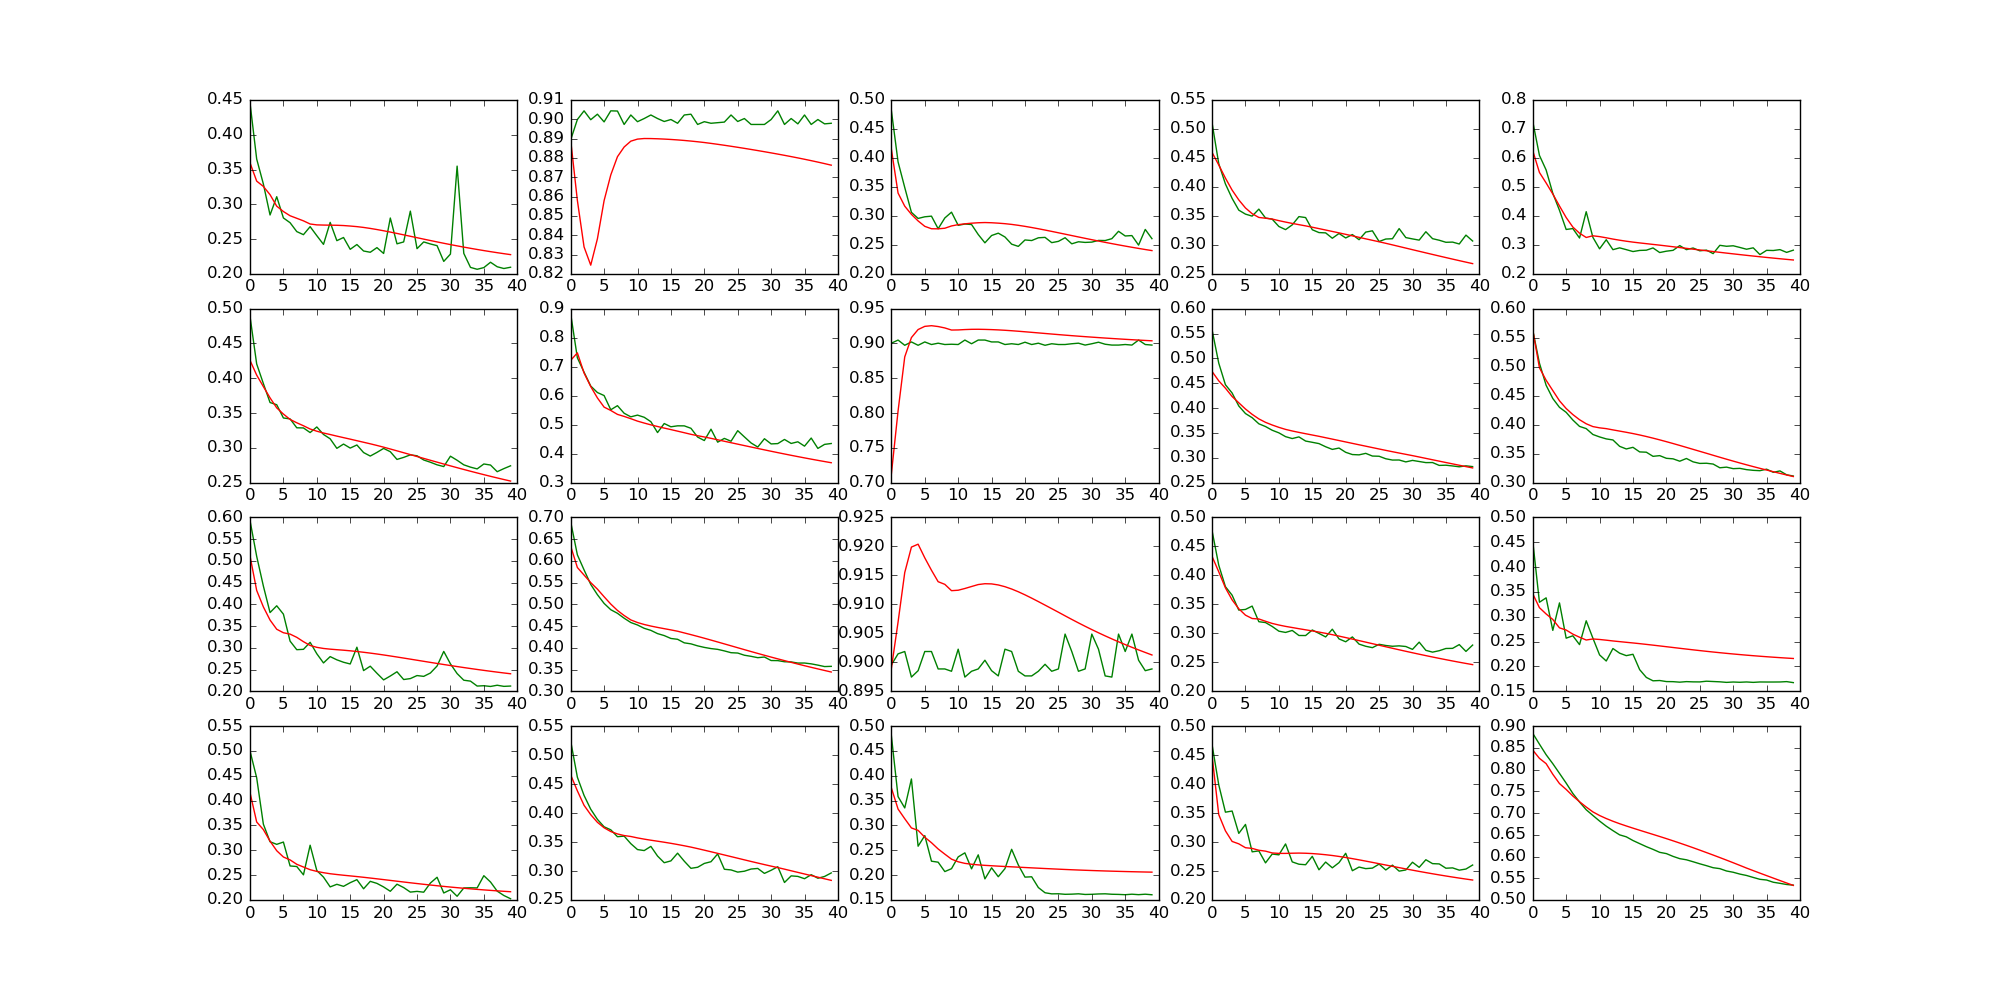
\includegraphics[width=1.2\textwidth]{../../figures/model01_rnd_f1_e869}


\end{document}